\documentclass [10pt]{article}
\textheight	8.7in
\textwidth	6.5in
\topmargin	    0in
\oddsidemargin  0in
\evensidemargin 0in
\baselineskip 15pt

\usepackage{amssymb,amsmath,amstext}
\usepackage{amsfonts}
\usepackage{mathtools}
\usepackage{tikz}
\usetikzlibrary{automata,arrows,calc,positioning}

\begin{document}
\title{Theory of Computation Assignment no. 3}
\author{Goktug Saatcioglu}
\date{}
\maketitle

\begin{enumerate}
	\item[\textbf{(1)}]Consider two copies of $DFA$ $M$ that recognizes the langauge $A$. From these two copies, say $M_{1}$ and $M_{2}$, we can consruct an NFA $M^{\prime}$ that recognizes $omission(A)$. Begin by making all accepting states in $M_{1}$ non-accepting and keep the initial state of $M_{1}$ as the initial state of $M^{\prime}$. The accepting states of $M^{\prime}$ are now going to be the accepting states of $M_{2}$. Then, for every transition $\delta(p_{1},a) = q_{1}$, where $a \in \Sigma$, in $M_{1}$ there is an equivalent state $q_{2}$ such that $\delta(p_{2},a) = q_{2}$ where $p_{2}$ is a copy of the state $p_{1}$ in $M_{2}$ and $q_{2}$ is a copy of the state $q_{1}$ in $M_{2}$. We can construct an NFA that recognizes $omission(A)$ by adding a $\lambda$-tranisiton for each $\delta(p_{1},a) = q_{1}$ from $p_{1}$ to its corresponding $q_{2}$ in $M_{2}$. If there are no transitions into $q_{0}$ in $M_{1}$ then remove the corresponding $q_{0}$ in $M{2}$ and otherwise convert the $q_{0}$ in $M_{2}$ to a non-accepting non-initial state. $M^{\prime}$ recognizes $omission(A)$ since the shift from $M_{1}$ to $M_{2}$ can only happen once, meaning only one letter $a$ can be removed from $w$ and still be able to recognize $u$ which is an omission of $w$.
	\item[\textbf{(2)}]
	\begin{enumerate}
		\item[a.]
		\begin{enumerate}
			\item[(ii)]
			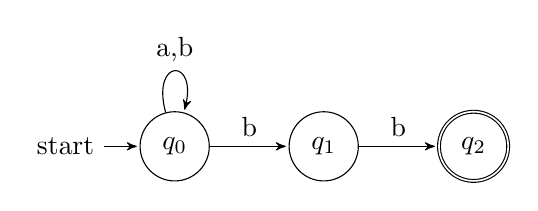
\begin{tikzpicture}[baseline=(q_0.north),>=stealth',shorten >=1pt, auto,node distance=1cm,align=center]
				\node[state,initial] (q_0) {$q_0$};
				\node[state] [right= of q_0] (q_1) {$q_1$};
				\node[state,accepting] [right= of q_1] (q_2) {$q_2$};
				\path[->]
					(q_0) edge [loop above] node {a,b} () 
					(q_0) edge node {b} (q_1)
					(q_1) edge node {b} (q_2);
			\end{tikzpicture}
			\\Where $q_{0} = \{w\:|\:w\in\Sigma^{*}\}$ (any word), $q_{1} = \{w\:|\:w\:\text{ends with}\:b\}$ (all words that end with $b$) and $q_{2} = \{w\:|\:w\:\text{ends with}\:bb\}$ (all words that end with $bb$).
			\item[(iii)]
			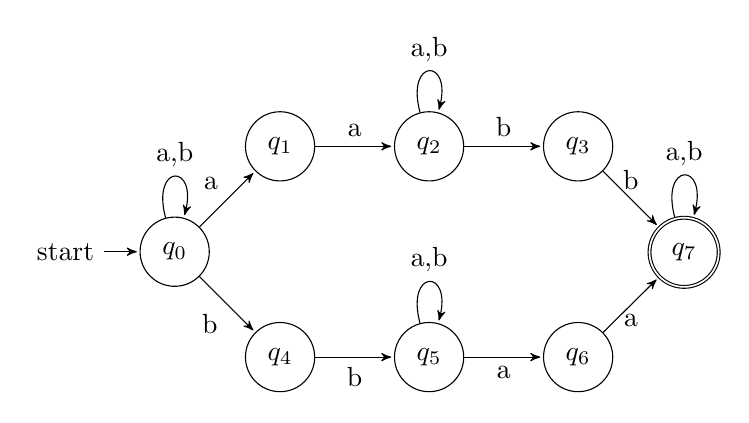
\begin{tikzpicture}[baseline=(q_0.north),>=stealth',shorten >=1pt, auto,node distance=1cm,align=center]
				\node[state,initial] (q_0) {$q_0$};
				\node[state] [above right= of q_0] (q_1) {$q_1$};
				\node[state] [right= of q_1] (q_2) {$q_2$};
				\node[state] [right= of q_2] (q_3) {$q_3$};
				\node[state] [below right= of q_0] (q_4) {$q_4$};
				\node[state] [right= of q_4] (q_5) {$q_5$};
				\node[state] [right=of q_5] (q_6) {$q_6$};
				\node[state,accepting] [below right= of q_3] (q_7) {$q_7$};
				\path[->]
					(q_0) edge [loop above] node {a,b} ()
					(q_0) edge node [above left] {a} (q_1)
					(q_0) edge node [below left] {b} (q_4)
					(q_1) edge node [above] {a} (q_2)
					(q_4) edge node [below] {b} (q_5)
					(q_2) edge [loop above] node {a,b} ()
					(q_2) edge node [above] {b} (q_3)
					(q_5) edge [loop above] node {a,b} ()
					(q_5) edge node [below] {a} (q_6)
					(q_3) edge node [above] {b} (q_7)
					(q_6) edge node [below] {a} (q_7)
					(q_7) edge [loop above] node {a,b} ();
			\end{tikzpicture}
			\\Where $q_{0} = \{w\:|\:w\in\Sigma^{*}\}$ (any word), $q_{1} = \{w\:|\:w\in\Sigma^{*}_{a}\}$ (all words that has $a$ as a substring), $q_{2} = \{w\:|\:w\in\Sigma^{*}_{aa}\}$ (all words that has $aa$ as a substring), $q_{3} = \{w\:|\:w\in\Sigma^{*}_{aa}\land w\in\Sigma^{*}_{b}\}$ (all words that have $aa$ and $b$ as substrings), $q_{4} = \{w\:|\:w\in\Sigma^{*}_{b}\}$ (all words that has $b$ as a substring), $q_{5} = \{w\:|\:w\in\Sigma^{*}_{bb}\}$ (all words that has $bb$ as a substring), $q_{6} = \{w\:|\:w\in\Sigma^{*}_{bb}\land w\in\Sigma^{*}_{a}\}$ (all words that have $bb$ and $a$ as substrings), and $q_{7} = \{w\:|\:w\in\Sigma^{*}_{aa}\land w\in\Sigma^{*}_{bb}\}$ (all words that have both $aa$ and $bb$ as substrings).
		\end{enumerate}
		\item[b.]If $L \in REG$ then there $\exists$ a DFA that identifies $L$. Let $M = (\Sigma, Q, q_{0}, F, \delta)$ be the DFA that identifies $L$. Then the DFA $M^{\prime} = (\Sigma, Q, q_{0}, Q \setminus F, \delta)$ identifies $L^{c}$. That is, $M^{\prime}$ is a DFA where the accepting and non-accepting states of $M$ are switched. Thus, if $L \in REG$ then $L^{c} \in REG$.
		\item[c.]If $L \in REG$, then there $\exists$ a DFA that idenfities $L$. Let $M = (\Sigma, Q, q_{0}, F, \delta)$ be the DFA that identifies $L$. We can then construct the following NFA $M^{\prime}$ by making the initial state of $M$ an accepting state, making all of the accepting states of $M$ non-accepting states, and reversing all transitions given by $M$. Furthermore, we introduce a new initial state, say $q_{0}^{\prime}$, that has $\lambda$ transitions from $q_{0}^{\prime}$ to the accepting states of $M$ (which have now become non-accepting states in $M^{\prime}$). Formally, $M^{\prime} = (\Sigma, Q^{\prime}, q_{0}^{\prime}, F^{\prime}, \delta^{\prime})$ where $Q^{\prime} = Q \cup \{q_{0}^{\prime}\}$, $F^{\prime} = \{q_{0}\}$ and $\delta^{\prime} = \{p \:|\: p \in \delta^{\prime}(q,a) \iff q \in \delta(p, a) \:\text{,where}\: p,q \in Q \:\text{and}\: a \in \Sigma \:\text{, and there are $\lambda$ transition from $q_0$ to the accepting states of $M$} \}$. Since the NFA $M^{\prime}$ identifies $L^{R}$, if $L \in REG$ then $L^{R} \in REG$.
	\end{enumerate}
	\item[\textbf{(3)}]
	\begin{enumerate}
		\item[a.]
		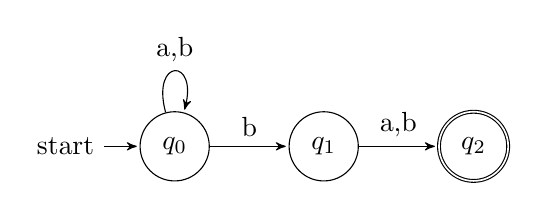
\begin{tikzpicture}[baseline=(q_0.north),>=stealth',shorten >=1pt, auto,node distance=1cm,align=center]
			\node[state,initial] (q_0) {$q_0$};
			\node[state] [right= of q_0] (q_1) {$q_1$};
			\node[state,accepting] [right= of q_1] (q_2) {$q_2$};
			\path[->]
				(q_0) edge [loop above] node {a,b} () 
				(q_0) edge node {b} (q_1)
				(q_1) edge node {a,b} (q_2);
		\end{tikzpicture}
		\\Where $q_{0} = w$ (any word), $q_{1} =$ a word that ends with $b$ and $q_{2} =$ a word where the 2nd from last letter is $b$.
		\item[b.]
		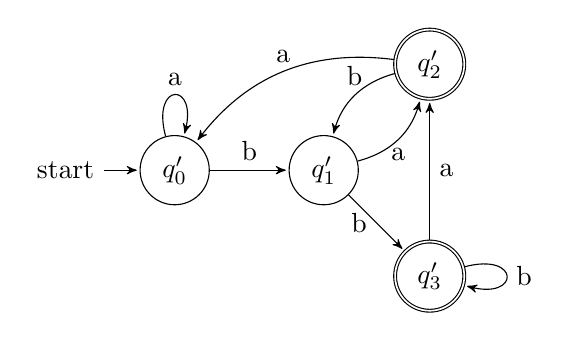
\begin{tikzpicture}[baseline=(q_0.north),>=stealth',shorten >=1pt, auto,node distance=1cm,align=center]
			\node[state,initial] (q_0) {$q_{0}^{\prime}$};
			\node[state] [right= of q_0] (q_1) {$q_{1}^{\prime}$};
			\node[state,accepting] [above right= of q_1] (q_2) {$q_{2}^{\prime}$};
			\node[state,accepting] [below right= of q_1] (q_3) {$q_{3}^{\prime}$};
			\path[->]
				(q_0) edge [loop above] node {a} ()
				(q_0) edge node {b} (q_1)
				(q_1) edge [bend right] node [below] {a} (q_2)
				(q_1) edge node [left] {b} (q_3)
				(q_2) edge [bend right] node [above] {a} (q_0)
				(q_2) edge [bend right] node [above] {b} (q_1)
				(q_3) edge [loop right] node [right] {b} ()
				(q_3) edge node [right] {a} (q_2);
		\end{tikzpicture}
		\\Where $q_{0}^{\prime} = \{q_{0}\}$, $q_{1}^{\prime} = \{q_{0}, q_{1}\}$, $q_{2}^{\prime} = \{q_{0}, q_{2}\}$ and $q_{3}^{\prime} = \{q_{0}, q_{1}, q_{2}\}$. States that are not denoted by prime are defined as above in (a).
		\item[c.]To create a DFA that identifies $L_{k}$ we can create a DFA, say $M_{k}$, with $2^{k}$ states where each state corresponds to one of the k-length words ($w$) that can be formed using $\Sigma^{*}$. Thus, our set of states, $Q_{k}$, is expressed as $Q_{k} = \Sigma^{k} = \{a,b\}^{k}$. This is because to identify $L_{k}$, $M_{k}$ must remember the last $k$ letters since the length of $w$ is not known beforehand. There are $2^{k}$ possible words of length $k$ and thus we need $2^{k}$ states that remember the last $k$ letterss of each word. For $M_{k}$ we use the transition function on a state when a letter $l^{\prime} \in \Sigma$ is read as a left shift operand where all letters in that state are shifted to the left by one and $l^{\prime}$ is concatenated to the end. Formally, if $l_{1}l_{2}...l_{k} \in \Sigma^{k}$ is a word of length $k$ and where $l_{i}$ denotes the position of a letter in that word, then $\delta_{k}(l_{1}l_{2}...l_{k}, l^{\prime}) = l_{2}l_{3}...l_{k}l^{\prime}$. The initial state would then be $q_{0} = a^{k}$ because any word with less than length $k$ cannot have a $b$ that is $k$'th from the last letter of that word Thus, we start with the word of all $a$'s of length $k$. Finally, the accepting states would be the set of all states that have a $b$ in the first position (i.e. $F_{k} = \{l_{1}l_{2}...l_{k}\:|\:l_{1} = b\})$). Overall, $M_{k} = (\Sigma, Q_{k}, q_{0}, F_{k}, \delta_{k})$ as described above.
		\item[d.]Suppose for the sake of contradiction that there exists a DFA $M$ that identifies the language $L$ with at most $2^{k-1}$ states. Since there are $2^{k}$ possible words of length $k$ by the pigeonhole principle there are two distinct $k$-length words $w_{1}$ and $w_{2}$ such that $M$ ends at the same accepting state when given the inputs $w_{1}$ and $w_{2}$. Pick any $i$ such that $w_{1}$ and $w_{2}$ are different from each other in the $i$'th position. Next, construct $w_{1}^{\prime} = wa^{k-i}$ and $w_{2}^{\prime} = wa^{k-i}$ such that $w_{1}^{\prime}$ and $_{2}^{\prime}$ contains a $b$ in the $k$'th position. We see that $w_{1}^{\prime}$ and $w_{2}^{\prime}$ end in the same accepting state when used as inputs for $M$. However, $M$, by our construction, is supposed to end at the same accepting state for exactly only two words which gives us a contradiction. Thus, $M$ must have at least $2^{k}$ states to identify $L$.
	\end{enumerate}
	\item[\textbf{(4)}]Let $N = (\Sigma,Q_{N},q_{N},F_{N},\delta_{N})$ be an NFA, and let $M = (\Sigma,Q_{M},q_{M},F_{M},\delta_{M})$ be its determinization as defined in class. We prove that for every $w\in\Sigma^{*}$, $\delta^{*}_{M}(q_{M},w)=\delta^{*}_{N}(q_{0},w)$ using induction on the length of $w$, say $n$.\\
	\textbf{Base case.} $n = 0 \implies \left|w\right| = 0 \implies w = \lambda$.
	\begin{align}
		\delta^{*}_{M}(q_{M},w) &= \delta^{*}_{M}(\{q_{0}\},\lambda) && \text{$w = \lambda,\: q_{M} = \{q_{0}\}$} \nonumber \\
		&= \{q_{0}\} && \text{by definition} \nonumber \\
		&= \delta^{*}_N(q_{0},\lambda) \nonumber \\
		&= \delta^{*}_N(q_{0},w) \nonumber
	\end{align}
	Since the LHS $=$ RHS the base case holds.\\
	\textbf{Inductive step.} For some $n \ge 0$, assume that $\delta^{*}_{M}(q_{M},w)=\delta^{*}_{N}(q_{0},w)$ where $\left|w\right| = n$. Now for $k = n$, consider a $w^{\prime\prime}$ such that $\left|w^{\prime\prime}\right| = k + 1$ and $w^{\prime\prime} = w^{\prime}a$, where $w^{\prime} \in \Sigma^{*}$ such that $\left|w^{\prime}\right| = k$ and $a \in \Sigma$. Now we evaluate $\delta^{*}_{M}(q_{M},w^{\prime\prime})$.
	\begin{align}
		\label{1} \tag{1} \forall p \in Q_{M}\quad\delta^{*}_{M}(p,wa) &= \delta_{M}(\delta^{*}_{M}(p,w),a) && \text{where $w \in \Sigma^{*}$ and $a \in \Sigma$}\\
		\label{2} \tag{2} \forall p \in Q_{N}\quad\delta^{*}_{N}(p,wa) &= \bigcup\limits_{q \in \delta^{*}_{N}(p,w)} \delta_{N}(q,a) && \text{where $w \in \Sigma^{*}$ and $a \in \Sigma$}\\
		\label{3} \tag{3} S \subseteq Q_{N}\quad\:\:\delta_{M}(S,a) &= \bigcup\limits_{q \in S} \delta_{N}(q,a) && \text{where $a \in \Sigma$}\\
		\delta^{*}_{M}(q_{M},w^{\prime\prime}) &= \delta^{*}_{M}(\{q_0\},w^{\prime}a) && \text{$w^{\prime\prime} = w^{\prime}a,\:q_{M}=\{q_{0}\}$} \nonumber \\
		&= \delta_{M}(\delta^{*}_{M}(\{q_{0}\},w^{\prime}),a) && \text{by property \ref{1}} \nonumber \\
		&= \delta_{M}(\delta^{*}_{N}(q_{0},w^{\prime}),a) && \text{by the induction hypothesis} \nonumber \\
		&= \bigcup\limits_{q \in \delta^{*}_{N}(q_{0},w^{\prime})} \delta_{N}(q,a) && \text{by property \ref{2}} \nonumber \\
		&= \delta^{*}_{N}(q_{0},w^{\prime}a) && \text{by property \ref{3}} \nonumber \\
		&= \delta^{*}_N(q_{0},w^{\prime\prime}) && \text{$w^{\prime}a = w^{\prime\prime}$} \nonumber
	\end{align}
	\textbf{Conclusion.} By the principle of induction, we see that for every $w\in\Sigma^{*}$, $\delta^{*}_{M}(q_{M},w)=\delta^{*}_{N}(q_{0},w)$ for $\left| w \right| = n$ where $n \ge 0$. $\Box$
	\item[\textbf{(5)}]Assume for the sake of contradiction that $A$ is regular. Then $A$ has a pumping constant $p$. Now consider the word $w = a^{p}b^{p+1}$ (i.e. there are $p$ $a$'s and $p+1$ $b$'s). Then we can write $w$ as $w = xyz$ such that the properties of the pumping lemma hold. By the property that states that $\left|xy\right| \le p$ and $\left|y\right| \ge p$, we can conclude that $y$ consists of only $a$'s (so does $xy$). By the lemma $xy^{n}z \in A\:\forall n \ge 0$, there exists a $w^{\prime} = xy^{2}z$ such that $w^{\prime} \in A$. However, since $\left|xy\right| \le p$ and $\left|y\right| \ge p$ there are now at least $p + 1$ $a$'s but we also still have $p + 1$ $b$'s. Therefore, for $w^{\prime}$ $\# a$'s $\ge \# b$'s and $w^{\prime} \notin A$. This is a contradiction to our initial claim that $A$ is regular and we conclude that $A$ is not regular.
\end{enumerate}

\end{document}